\documentclass{mpaper}

\usepackage{graphicx}
\usepackage{multirow}
\usepackage{booktabs}
\usepackage[format=plain, labelfont={bf},textfont=it,tableposition=above]{caption}
\usepackage{siunitx}

\begin{document}

\title{mmFace: 3D Face Recognition with RGB and Millimetre Wave Radar}
\author{Stergious Aji}
\matricnum{2546916A}

\maketitle

\begin{abstract}
    TODO
    % According to Simon Peyton Jones, an abstract should address four key questions. First, what is the problem that this paper tackles? Second, why is this an interesting problem? Third, what is the solution this paper proposes? Finally, why is the proposed solution a good one?


\end{abstract}

% This paper outlines the standard template for a final MSci project report submission at the School of Computing Science in the University of Glasgow. In earlier years, MSci students at the School of Computing Science\footnote{\url{https://www.gla.ac.uk/computing}}, University of Glasgow, were expected to produce a full-length dissertation. Now, the requirement is for MSci students to write a paper of up to 14 pages in length, using the supplied \texttt{mpaper} \LaTeX style file.

% The precise structure of an MSci paper is not mandated, but it should probably cover in detail the following aspects of the project.
% \begin{enumerate}
% \item General description of the problem, motivation, relevance
% \item Background information, possibly including a literature survey
% \item Description of approach taken to solve the problem, including high-level design and lower-level implementation details as appropriate
% \item Evaluation, qualitative or quantitative as appropriate
% \item Conclusion, including scope for future work
% \end{enumerate}

\section{Introduction}
% Facial recognition technology is a key area of research within the field of computer vision, with widespread applications across areas such as security surveillance, forensic analysis, and human-computer interaction. Its most prominent use case lies in biometric authentication, allowing individuals access to their personal devices or restricted areas. This enables a non-invasive, hands-free approach to identity verification, removing the need to recall passwords. Furthermore, facial biometrics are naturally more accessible than other forms such as fingerprints, iris, or palm prints \cite{zhou20183d}.
Facial recognition is an evolving research domain within the field of computer vision, finding extensive use across areas including human-computer interaction, security surveillance, and forensic analysis. Its primary application revolves around biometric authentication, granting individuals access to their devices or restricted zones. This enables a non-intrusive, hands-free means of verifying identity, eliminating the need to memorise passwords. Additionally, facial biometrics are naturally more attainable than other modalities such as fingerprints, palm prints, or iris scans \cite{zhou20183d}.

% Since its inception in the 1960s, facial recognition systems have evolved drastically. The pioneering work by Bledsoe \cite{bledsoe1966model} first distinguished faces by comparing distances of manually annotated landmark features such as the nose, eyes, and mouth. In more recent years, the advent of deep learning has enhanced the performance and efficiency of human face classification, benefitting from the vast online repositories of face images.  Nevertheless, these systems primarily rely on images captured by RGB cameras, making them susceptible to variations in lighting and pose \cite{xu2004depth}. By incorporating depth data, which draws attention to the geometric details of the face, the effect of such environmental factors can be mitigated. Moreover, the transition to three-dimensional face recognition not only improves accuracy, but also enhances the security of biometric systems against spoofing attacks \cite{wen2015face}.
Since its inception in the 1960s, facial recognition technology has undergone significant growth. Initially pioneered by Bledsoe \cite{bledsoe1966model}, early systems distinguished faces by comparing manually annotated landmark features such as the nose, eyes, and mouth. In recent years, the emergence of deep learning has reshaped human face classification, leveraging extensive online repositories of face images for improved performance and efficiency. However, these systems predominantly rely on images captured by RGB cameras, leaving them vulnerable to variations in lighting and facial pose \cite{xu2004depth}. By incorporating depth data and drawing attention to the geometric details of the face, the impact of such environmental factors can be regulated. Furthermore, the transition to three-dimensional facial recognition not only increases accuracy but also bolsters the security of biometric systems against spoofing attacks \cite{wen2015face}.


\subsection{Motivation}
% The popularity of 3D face recognition is on the rise, evidenced by its adoption in smartphones with the likes of Apple and their Face ID \cite{apple-faceid} technology. This growing demand has pushed the commercialisation of depth-sensing technology to smaller form factors, enabling it to operate efficiently in real-time on mobile devices \cite{soumya2023recent}. Face ID, in particular, has achieved a level of security that allows its integration into services like Apple Pay. However, the use of costly proprietary hardware and restrictive patents by Apple make it harder for smaller companies to adopt an equally compact and secure face recognition system.
The popularity of 3D face recognition is on the rise, evidenced by its adoption in smartphones with the likes of Apple and their Face ID \cite{apple-faceid} technology. This growing demand has pushed the commercialisation of depth-sensing technology to smaller form factors, facilitating its efficient real-time operation on mobile devices \cite{soumya2023recent}. Face ID, in particular, has garnered a level of security that enables payment authentication within services such as Apple Pay. However, Apple's use of costly proprietary hardware and restrictive patents make it harder for smaller companies to adopt an equally compact and secure face recognition system.

% Depth cameras used in this context typically employ an active acquisition method. This is where non-visible light is projected onto the face and reflected back, allowing sensors to measure and map facial features. The most common approach involves lidar cameras, emitting waves in the near-infrared (NIR) spectrum, due to their ability to capture a dense 3D map of the subject's face \cite{wang2020evolution}. However, its weakness in penetrating materials such as clothing and hair is a notable limitation. In contrast, millimetre radar waves (mmWaves) can penetrate such materials to directly reach the dermal layer of the skin \cite{vizard2006advances}, potentially offering better performance in scenarios involving facial hair, or even within challenging environmental conditions such as rain or fog.
Depth cameras, used in this context, typically employ an active form of acquisition. This involves projecting non-visible light onto the face, which is then reflected back, allowing sensors to gauge and delineate facial features. Lidar cameras, emitting waves in the near-infrared (NIR) spectrum, are the most prevalent choice given their capacity to acquire a dense 3D map of the subject's face \cite{wang2020evolution}. However, they are limited by their inability to penetrate thin materials such as clothing and hair. In contrast, millimetre wave radar (mmWaves) can penetrate such materials and directly reach the skin's dermal layer \cite{vizard2006advances}. This could enable greater performance in scenarios involving facial hair or adverse environmental conditions such as rain or fog.

% Research into the efficacy of radar waves for 3D face recognition is relatively sparse, but recent studies show positive results \cite{hof2020face, lim2020dnn,kim2020face, pho2021radar, challa2021face}. Radar sensors are generally more cost-effective, both in terms of acquisition and computation, as they consume less power compared to NIR-based sensors. However, it is important to note the trade-off, as mmWaves tend to yield a sparser, less accurate representation in comparison. This could impact recognition performance where precision in detecting and mapping facial features is paramount. This project aims to therefore explore counter-balancing this limitation with the information gained from colour images, potentially paving the way for more resilient and versatile systems. 
Research into the efficacy of radar waves for 3D face recognition remains relatively limited, although recent studies indicate promising outcomes \cite{hof2020face, lim2020dnn,kim2020face, pho2021radar, challa2021face}. Radar sensors typically offer greater cost efficiency in terms of both acquisition and computation, as they consume less power compared to sensors NIR-based systems. Nevertheless, it is crucial to acknowledge the trade-off, as mmWaves often result in a sparser representation. This could impact recognition accuracy, where precision in detecting and mapping of facial features is paramount. Thus, we aim to address this limitation by integrating information from colour images, potentially paving the way for more resilient and versatile systems.


\subsection{Research Aims}
Our work explores the effectiveness of using RGB cameras in conjunction with mmWave radar sensors for 3D facial recognition. Since there are no appropriate datasets available for this purpose, we have collated this data ourselves. We use the Intel RealSense L515 RGB-D camera \cite{intel-l515} for photographing an individual's face. Meanwhile, the Google Soli \qty{60}{\GHz} radar sensor \cite{lien2016soli} is employed to gather depth information by transmitting and measuring millimetre waves reflected from the target.

We initially planned to gather face data from approximately \num{50} participants, however, only \num{21} participants came forward within the limited timeframe. We obtained face data under various conditions including diverse poses, lighting environments, and common occlusion scenarios. This approach yielded a system that is invariant to environmental conditions in comparison to RGB-only systems.

We developed a novel face recognition model using a deep convolutional neural network. This model was trained on the captured data in order to learn facial features from both the RGB and depth characteristics acquired from the Soli sensor, simultaneously. We investigated different techniques in fusing these two modalities, aiming to pinpoint the most effective strategy that provides rich and distinctive representations, for clean identity separation. The model's effectiveness is benchmarked against prior radar-based facial recognition systems, as well as, a comparison to solely using RGB data.

The main contributions of this paper are listed below:

\begin{enumerate}
    \item Explore the feasibility of using RGB cameras in conjunction with mmWave radar sensors for 3D facial recognition.
    \item Collated a face dataset of colour images and mmWave signatures from a diverse array of 21 participants. The Intel Realsense L515 \cite{intel-l515} and the Google Soli chip \cite{lien2016soli} will be employed to accomplish this. This data will be obtained under various conditions including diverse poses, lighting environments and common occlusion scenarios.
    \item Empirically test the hypothesis that incorporating the depth information from the mmWave face signatures yields a more robust system, invariant to pose, lighting, occlusion, and spoofing.
    \item Develop a novel face recognition model that can be trained on both modalities simultaneously. This model should be able to classify a given face as well as identify if it is live or fake. OPEN SOURCE GITHUB
    \item Investigate various feature fusion methods to determine the optimal approach for integrating the RGB and mmWave facial features. This aims to yield richer, more distinctive representations for better face classification performance.
    \item Investigate the proposed model's effectiveness at classifying unseen faces and identifying their liveness compared to solely using RGB data.
\end{enumerate}



\section{Background}
\subsection{mmWave Radar Technology}
Radio Detection and Ranging, or Radar, has been around for decades and is instrumental in fields such as space exploration, military and commercial aviation, as well as maritime navigation. Recently, the miniaturisation of radar sensors to the millimetre wave band has brought its application to more small-scale domains \cite{soumya2023recent}. mmWave sensing has been very successful in the domain of autonomous vehicles for object detection, specifically in systems such as collision warnings and adaptive cruise control \cite{dfrobot}. This is primarily due to its edge over traditional near-infrared waves employed by lidar cameras, particularly in its resilience to atmospheric conditions such as dust, smoke, fog, and rain \cite{cadenceblog2022}. This penetrative power of mmWaves make it a promising candidate for reliable facial recognition in uncertain, real-world scenarios. 

Another notable example is Google's integration of their Soli sensor into the Pixel 4 smartphones for motion detection and gesture recognition \cite{googleblog2020}. However, its application to face recognition is unexplored offering a unique research area. Consequently, this is the sensor we used to capture mmWave face signatures during our data collection phase. A key driving factor for this choice is the Soli's miniature form factor of just \qty{6.5}{\mm} $\times$ \qty{5.0}{\mm}, portability, and its use of Frequency Modulated Continuous Wave (FMCW) technology. This is proven to offer superior range resolution in comparison to other modulation techniques due to its high pulse compression \cite{mahafza2005radar}, a vital aspect for extracting accurate facial features. The Soli chip has a relatively low power consumption due to the fact that it sends 16 chirps every burst at a pulse-repetition frequency of \qty{2}{\kHz}, then stops transmitting until the next burst of chirps \cite{hayashi2021radarnet}. Each burst is transmitted at \qty{25}{\Hz} giving an overall transmission duty cycle of 2\% meaning the radar chip is turned off during the majority of its operation saving a lot of power for mobile applications.


% However, it is important to note the trade-off, as mmWaves tend to have a lower accuracy in comparison. This could impact face recognition performance where precision in detecting and mapping facial features is paramount. This project will therefore explore counter-balancing this limitation with the information gained from RGB images, potentially paving the way for more resilient and versatile systems.


\subsection{Related Work}
The use of millimetre waves for face identification is a relatively new research field, spurred by the commercialisation of radar sensor technology. One of the earliest studies found to investigate human identification using mmWaves can be traced back to 2019, conducted by Zhao et al. \cite{zhao2019mid}. Although this paper focuses on classifying subjects by their gait and body shape rather than facial features, it demonstrates the ability of mmWaves to encapsulate the subtle idiosyncrasies among individuals. These nuanced differences are vital for learning models to effectively differentiate between unique subjects, leading to high classification accuracies.

Following this, Hof et al. \cite{hof2020face} proposed a Deep Neural Network (DNN) based Autoencoder that can distinguish human faces captured by an 802.11ad/y networking chipset operating at a centre frequency of 60 GHz. The Autoencoder is able to encode mmWave face signatures of over 200 individuals with enough separation to distinguish between positive and negative instances by measuring their Mean Squared Error (MSE) against reference facial embeddings. The study conducted an extensive data collection process, capturing face scans of 206 participants comprising various genders and ages, in five different poses: frontal, as well as, $15^\circ$ and $25^\circ$ head rotations to the left and right. This collection was subsequently made available through an IEEE Data Port \cite{mmwavefacedata}. While this dataset encapsulates faces from a wide range of people, including some with beards and spectacles, it lacks representation of other common occlusion scenarios like head accessories, that our project aims to explore. Moreover, the study utilised a larger sensor containing a total of 1024 transmit and receiver antenna pairs, found to capture redundant information. This is in contrast to the compact Soli chip with a single transmit and three receiver antennas, intended to work within a smartphone. The study simulated the effect of reducing the antenna count to 10, markedly decreasing the distinctiveness of facial signatures. Promisingly, increasing the number of neurons in their Neural Network and an additional hidden layer could compensate for this reduction, maintaining high accuracy.

Lim et al. \cite{lim2020dnn} proposes another Deep Neural Network model, however with a more traditional Multi-Layer Perceptron (MLP) architecture where every layer is fully connected to adjacent ones. The study utilised a small-scale, 61 GHz FMCW radar sensor developed by bitsensing Inc. \cite{bitsensing2020bts60}, comparable to the Google Soli with a single transmit and three receiver antennas. The model attained a mean classification accuracy of 92\% across eight subjects, surpassing the performance of both, a Support Vector Machine (SVM), and a tree-based Ensemble Learning approach trained on the same face signatures. It is important to note the relatively small-sized dataset used to train the model, raising concerns about potential overfitting as the data is not representative enough. The paper provides limited details on the data collection methodology used, only mentioning that the facial distances ranged from 30 cm to 50 cm. It can be assumed then that the study likely focussed on frontal poses without any occlusions for all eight subjects. The research also explored the impact of using a single receiving antenna, which resulted in a reduced accuracy of 73.7\%. This finding is in line with Hof et al.'s \cite{hof2020face} observation that an increased number of receiving antennas can enhance classification accuracy by the ability to capture more nuanced facial features. The paper also suggests that a CNN may be more appropriate if signals were stacked on the time axis rather than the frequency axis.

During the same period, Kim et al. \cite{kim2020face} conducted research using an identical 61 GHz FMCW radar sensor from bitsensing Inc., featuring a range resolution of 2.5 cm. Their study introduces a CNN model comprising three convolutional layers and three fully connected layers. The radar data underwent heavy preprocessing to transform it into a more image-like format suitable for the CNN model. With a data split of 70\%/15\%/15\% for training, validation, and testing, the model achieved an average classification accuracy of 98.7\% on a limited dataset of only three individuals. Interestingly, the study also examined the impact of wearing cotton masks. The results showed a minimal drop in average classification accuracy by 0.9\%, which is encouraging for the objectives of our project. However, these findings are to be taken with caution due to the small size of the dataset. It remains unclear whether this level of performance would hold consistently across a larger and more diverse group of subjects, with more varied occlusions.

Pho et al. \cite{pho2021radar} adopts a One-Shot Learning approach to the problem. This is where the model is trained with a single or only a few labelled instances, beneficial when there is a lack of training samples available. The proposed method constitutes a Siamese structure of two identical CNNs with shared parameters that map the input radar signals into a latent space. A distance metric between the outputs of both CNNs is used during the training and testing phases to measure the similarity between face inputs. The model is specifically trained for \textit{binary classification} by inputting pairs of face signatures from either the same or different people. This process resulted in the model learning embeddings that push different faces into distinct Euclidean regions of the embedding space. The same bitsensing Inc. BTS60 chipset, used by Lim et al. and Kim et al. \cite{lim2020dnn, kim2020face}, is employed to capture 500 frames of the faces of eight participants. An average classification of 97.6\% was achieved, an improvement over the previous DNN model by Lim et al. involving the same number of people. t-Stochastic Neighbour Embedding (t-SNE) \cite{van2008visualizing} is then applied for dimensionality reduction. The resulting visualisations demonstrated that the one-shot Siamese network effectively separated each individual's face into exclusive regions, simplifying the classification task. Although a small dataset is used,\,only encompassing frontal poses with no occlusion\,settings, the proposed method is well documented and is likely robust against larger datasets.

Challa et al. \cite{challa2021face} employs two different machine learning models on the dataset made available through the IEEE port \cite{mmwavefacedata}. Their approach began with CNN-based Autoencoders followed by a Random Forest Ensemble Learning approach. A total of nine Autoencoders were built, each tailored to different frame rates, focusing on compressing and learning to reconstruct the original data from its compressed, latent form. The Autoencoders were trained using randomly selected data samples from a subset of 186 mmWave face signatures. The flattened and labelled outputs were then used to train and test nine discrete Random Forest models using identical hyperparameters, as recommended by the Sci-kit library. This methodology yielded impressive results, achieving an average classification accuracy of 99.98\% using all 1400 frames per individual. Even reducing the number of frames to 70 per person, the model was able to maintain a high accuracy of 97.1\%. The paper presents an approach that is unique in comparison to the rest of the research papers tackling this subject, showcasing an efficient model that is able to be deployed on mobile chips.

The research in this area exclusively focuses on utilising data from radar sensors, largely driven by concerns of privacy preservation. However, a significant limitation of this approach is the required duration for capturing an accurate facial scan. The sensor needs to operate for several seconds, typically in the range between 10 and 15 seconds, in order to obtain a detailed scan. Such a time frame is impractical in real-world situations, as it necessitates the subject to remain motionless for a prolonged period. Up to this point, no study was found to explore the potential benefits of combining radar signatures with corresponding RGB data to enhance facial recognition capabilities. Given the high performance of existing deep learning models using RGB images alone, such as InsightFace \cite{deng2018arcface}, integrating these models with mmWave radar data presents a promising avenue. This combination could accelerate face acquisition time, while leveraging the advantages of mmWaves in terms of their robustness to lighting variations and occlusions.


\subsection{InsightFace}
\label{background:insightface}
In the evolving field of face recognition, deep CNNs have emerged as a dominant approach due to their ability to extract discriminative facial features from images. One significant advancement in this area is the InsightFace toolkit, implementing algorithms designed to address the intricacies of face analysis and recognition. Key works include the preliminary ArcFace model, introduced by Deng et al. \cite{deng2018arcface}, alongside the robust Face Alignment model by Gho et al. \cite{guo2018stacked}. ArcFace employs a novel Additive Angular Margin Loss to maximise class separability, further enhancing the discriminative power in mapping face images to feature embeddings. However, this method was found to face challenges with label noise, requiring the ``cleaning'' of many real-world images sourced from the web. To address this, further progress was made with the Sub-center ArcFace model \cite{deng2020subcenter}, introducing the concept of sub-classes to boost resilience against intra-class variations and label noise. It achieved state-of-the-art performance on many widely used benchmark datasets such as the Labeled Faces in the Wild (LFW) \cite{huang2008labeled} and the YouTube Faces (YTF) datasets \cite{wolf2011face}.

The integration of pretrained models offered by InsightFace into our system enables us to concentrate primarily on enhancing the performance of our CNN learning mmWave face signatures. By fusing the depth and contour detection capabilities of mmWave radar with the rich, textural features gathered by ArcFace from RGB images, the system has the potential to attain improved accuracy and robustness. This approach is particularly promising in environments where conventional optical methods falter.


\subsection{Multimodal Data Fusion Techniques}
\label{background:multimodal_data_fusion_techniques}
Multimodality, as defined by Lahat et al. \cite{lahat2015multimodal}, refers to the use and analysis of multiple types of data, potentially arriving from multiple sensors. The aim is to extract and blend salient information gathered by each sensor. The integration of this diverse data lead to outputs with richer representations than what could be achieved by the individual modalities alone. We hypothesise that coupling the colour information from face images with the depth gathered by the radar sensor could greatly improve class separation, and subsequently, face recognition performance.

A common technique involves fusing the multiple data modalities before feeding them into a learning model, referred to as \textbf{Early Fusion}, or \textbf{Data-level Fusion}. It includes combining data by removing correlations between sensors or fusing data in a common, lower-dimensional space \cite{khaleghi2013multisensor}. Techniques such as Principal Component Analysis (PCA) and Canonical Correlation Analysis (CCA) are commonly employed for this purpose. One key issue with applying early fusion is ensuring synchronisation between the RGB and radar frames, which is difficult due to their significantly different sampling rates. Furthermore, the continuous mmWave signals must be effectively discretised to match the form of the RGB data. A major disadvantage of early fusion is the potential to squash critical information present within each individual modality, impacting the training efficacy.

\textbf{Late Fusion}, or \textbf{Decision-level Fusion}, operates by independently processing different data sources through separate models and then fusing them at the decision-making stage. A standard approach involves taking a weighted average of the separate predictions, providing a way to minimise or maximise the influence of specific modalities \cite{pawlowski2023effective}. Late fusion is often simpler and more flexible, and it can be effective when dealing with extremely dissimilar data sources either in terms of sampling rate, dimensionality, or unit of measurement. Additionally, late fusion often yields better performance since errors from multiple models are dealt with independently.

\textbf{Intermediate Fusion} or \textbf{Feature-level Fusion} is based on DNN architectures and involves the idea of combining different modalities within the feature space where there is a higher level of abstraction of the raw data. This can be as straightforward as a simple concatenation of the individual latent embeddings, or as complex as using Autoencoders for non-linear feature fusion \cite{charte2018practical}. This approach offers greater versatility than early and late fusions, as it allows for the integration of features at various depths within the neural network. However, it can lead to challenges such as a risk of overfitting or a failure in learning relationships between the different modalities.

Each data fusion technique comes with its own set of challenges and considerations, necessitating experimentation to determine the most effective way to merge the RGB and mmWave signatures. A variant of late, feature-level fusion is the most feasible where the embeddings from the last layers of each model are combined. It would be challenging to attempt early fusion due to the substantial differences between the two modalities. Such integration would likely require heavy preprocessing of the radar data, potentially involving its conversion into a depth image-like format. 



\section{Methodology}

\subsection{Data Acquisition and Experiments}
Following a thorough research of the field, the next steps involve designing and conducting the data acquisition process necessary to train our proposed model with. These experiments require careful planning since the data collected here directly determines the effectiveness of the resulting model. As found in Section \ref{background:data_acquisition} of the Background, it is vital to compile multiple poses in order for the model to learn a comprehensive 3D scan of the individual's face. Furthermore, it induces pose-invariance into the system, accommodating real-world use cases where individuals may not always present an exact frontal pose to the face recognition system. Most studies concentrate on variations in the yaw axis since a person is less likely to tilt or pitch their head by a significant angle in comparison to left and right rotations of the face. For this reason, we will similarly focus on head rotations around the yaw axis. We plan to record facial poses at $0^\circ$, as well as, $30^\circ$ and $45^\circ$ to the left and right of the sensors, denoted by positive and negative angles. 

Since this experiment aims to explore the benefits of mmWave sensors in the context of face recognition, two different lighting conditions will be incorporated in our data collection experiments. Namely, regular and dim lighting scenarios. We hypothesise that the mmWave face signatures would be unaffected by environmental lighting due to the sensor using its own active illumination of the target face, unlike the RGB camera. Therefore, if the system is able to demonstrate higher accuracy utilising both modalities as opposed to relying solely on RGB data, it would conclusively show that mmWaves offer robustness against varying lighting conditions.

Finally, we aim to investigate the penetrative power of mmWaves to directly reach the skin through cloth and hair by injecting common occlusion scenarios into our experiments. It would be beneficial for facial recognition systems to be robust against typical obstructions such as glasses, hats, masks and so on. Currently, users would be required to remove such accessories for systems to accurately identify and grant them access to particular devices or areas. With mmWaves, we hypothesise that this may not be needed since facial features could be captured regardless. This could greatly benefit security surveillance where individuals deliberately obscure their faces in order to hide their identities. In our experiment, we aim to capture scenarios both with and without occlusion. Since cotton masks have already been explored by Kim et al. \cite{kim2020face}, other common items like hats, sunglasses, and scarves will be used to mirror day-to-day scenarios.

On top of investigating environmental invariances, our research seeks to determine the least amount of radar data necessary to still yield easily separable facial embeddings. Previous studies were observed to record between 200 and 2,000 total frames which, depending on the sampling rate, requires running the sensor for eight to a maximum of 80 seconds for each scenario. This is due to the lower accuracy of mmWaves demanding a longer exposure to provide a dense enough representation. Nevertheless, requiring an individual to keep their face still for over three seconds is impractical in real-world applications. Our approach, which integrates RGB data, may reduce the need for prolonged radar frame capture. Consequently, in our experiments, we will collect 10 RGB frames and a maximum of 250 frames worth of mmWave bursts, equivalent to operating the Google Soli sensor for 10 seconds at a 25 Hz sampling rate. This approach will provide ample data to assess the minimum number of mmWave frames needed for effective identification. 

To ensure a diverse range of facial data, we aim to recruit 50 participants, given the tight timeframe of this project. Adhering to ethical standards regarding sensitive personal information, our participant pool will consist of adults, predominantly university students. While this results in an over-representation of individuals aged 20--25 years, it should not impact our study as age variance is not something that is being explored. A total of 15 scenarios will be captured for each participant at a distance of 20 cm from the sensors. Each time the sensors will be run for 10 seconds, totalling 150 RGB frames and 3,750 mmWave frames per person.

\begin{figure}[h!]
    \centering
    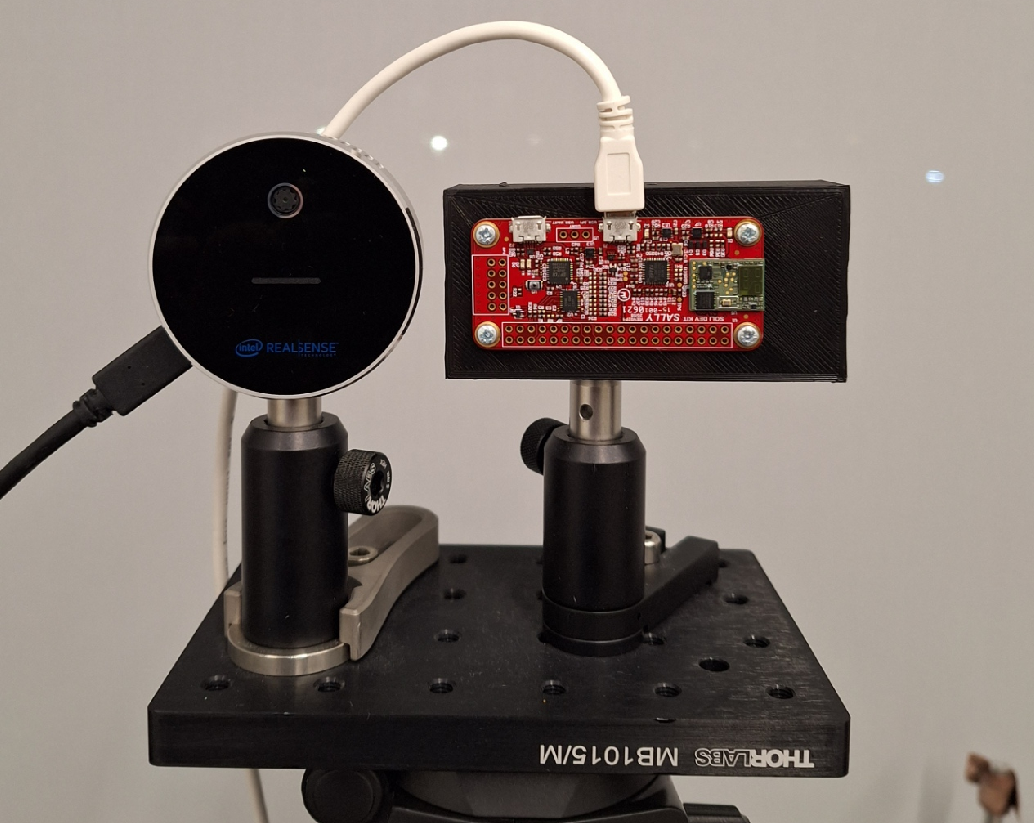
\includegraphics[width=0.35\textwidth]{diagrams/equipment.pdf}
    \vspace{0.2cm}
    \caption{Equipment: Intel Realsense L515 RGB-D Camera (Left) and the Google's Soli 60 GHz radar sensor (right)}
    \label{fig:equipment}
\end{figure}

\begin{figure}[h!]
    \centering
    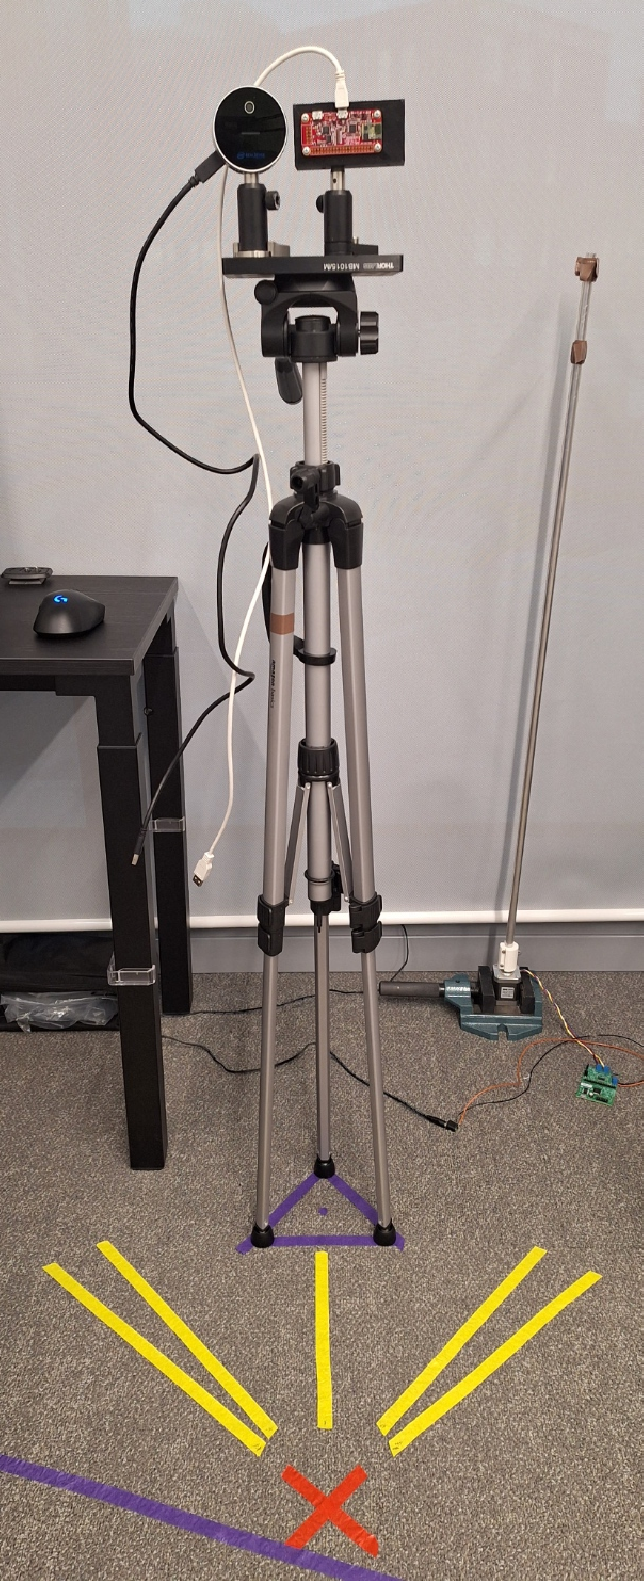
\includegraphics[width=0.31\textwidth, height=12.5cm]{diagrams/experiment_setup.pdf}
    \caption{Experiment Setup}
    \label{fig:experiment_setup}
\end{figure}


\subsection{mmFace}
Building on the intuition from Section \ref{background:insightface} of the Background chapter, it is clear that the ArcFace model from the InsightFace toolkit emerges as the best choice for our project. It attains state-of-the-art classification results on accepted benchmark sets, outperforming the previous bests such as Facebook's DeepFace \cite{taigman2014deepface} and Google's FaceNet \cite{schroff2015facenet}. This selection allows us to treat the RGB data processing as a \textit{black-box} framework, enabling us to concentrate efforts on perfecting the radar-based model we are naming, \textit{mmFace}. Furthermore, this facilitates exploration into the various methods in fusing the two modalities as discussed in Section \ref{background:multimodal_data_fusion_techniques}. Figure \ref{fig:model_architecture} shows a high-level diagram of the model workflow described here. 

Our proposed model, mmFace, will employ a CNN-based architecture, which is particularly effective for processing image-like data. The radar bursts obtained during the data collection phase will be transformed into Complex Range-Doppler (CRD) maps \cite{lien2016soli,hayashi2021radarnet} prior to feeding it into the model. Face scans will be collected using the Google Soli's short configuration which operates at a centre frequency of 60 GHz, with a maximum bandwidth $B$ of 5.5 GHz, and bursts sampled at 25 Hz. This gives a range resolution of $\frac{c}{2B} = 2.7$ cm, where $c$ denotes the speed of light. Given that the Intel RealSense captures RGB-D frames at a different sampling rate of 30 frames per second (FPS), timestamp information is also recorded for the possibility of synchronising the two modalities for early data fusion.

TODO:
The Soli chip as single transmit antenna and three receiver antennas capturing a superposition of scattered reflections from the target

As explained before, the data fusion techniques we plan to investigate include late, feature-level fusion and late, decision-level fusion. Pure intermediate fusion is not feasible due to the black-box treatment of the InsightFace model making it difficult to integrate information from both modalities within its hidden layers. Nonetheless, late, feature-level fusion remains viable, combining the outputs of the final layers of each model to form an embedding containing both the RGB and radar features. Similarly, decision-level fusion will be explored since this entails mixing the predictions from the individual models. Early fusion presents significant challenges due to the dissimilarities in sampling rates and data formats of the two modalities. The CRD maps must be synchronised and transformed into a depth image-like format before merging with the RGB images. Furthermore, this would require a whole new training cycle with the mmFace model which may be infeasible within the project's timeframe. However, should time permit, we will consider investigating this approach.

We plan to adopt a ResNet-based architecture for mmFace due to its refinements over its predecessors like AlexNet \cite{krizhevsky2012imagenet} and VGGNet \cite{simonyan2014very}. The ResNet framework \cite{he2016deep} incorporates ``skip connections'' and residual blocks to resolve the vanishing gradient problem encountered in VGGNet, allowing scaling of the network beyond the 19-layer limitation. This support for deeper networks provides a strong foundation for the mmFace model for learning the complex radar face signatures.

The dataset, comprising 50 participants, will be divided by subjects into an $80\%/10\%/10\%$ split for training, validation, and testing. Given the dataset's small size, a larger proportion is allocated for training to ensure the model can learn effectively. Following training, the testing phase will evaluate the distinctiveness of the output face embeddings. For accurate classifications, each person's face must be spatially separable in the high-dimensional embedding space allowing for unambiguous identification. t-SNE visualisations \cite{van2008visualizing} will be employed to visually inspect and confirm this is the case by comparing against the original data. In addition, standard classification accuracies will be calculated to verify the model's identity recognition capabilities against randomly selected ground truths. This also allows benchmarking our results against previous studies on radar-based 3D facial recognition.


\subsection{Feature-Level Fusion}


\begin{figure*}[h!]
    \centering
    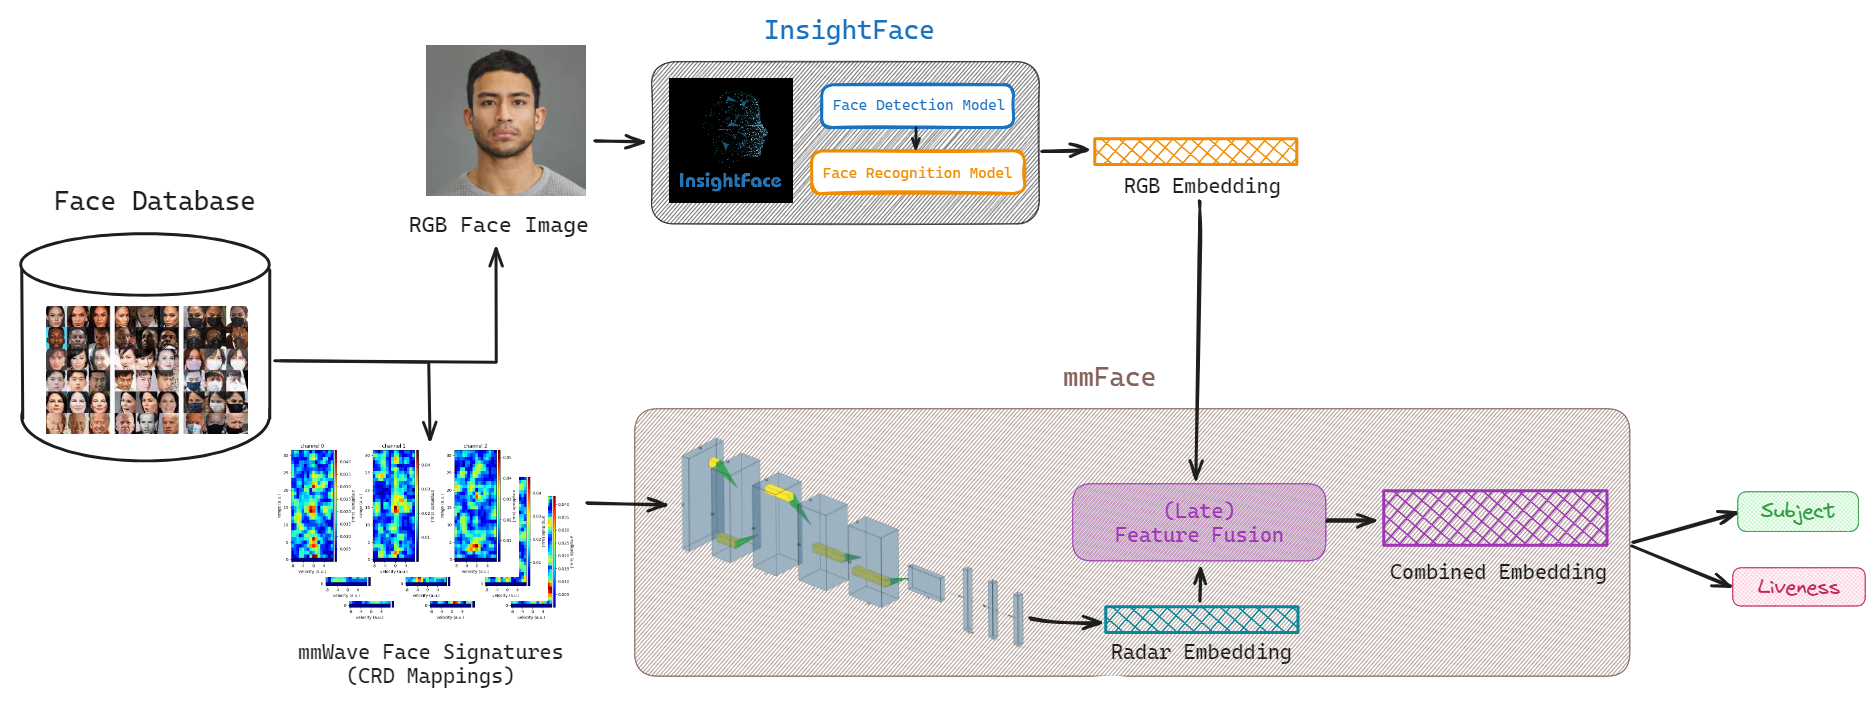
\includegraphics[width=1\textwidth]{diagrams/model_workflow.png}
    \caption{Workflow Diagram}
    \label{fig:model_workflow}
\end{figure*}

\begin{figure*}[h!]
    \centering
    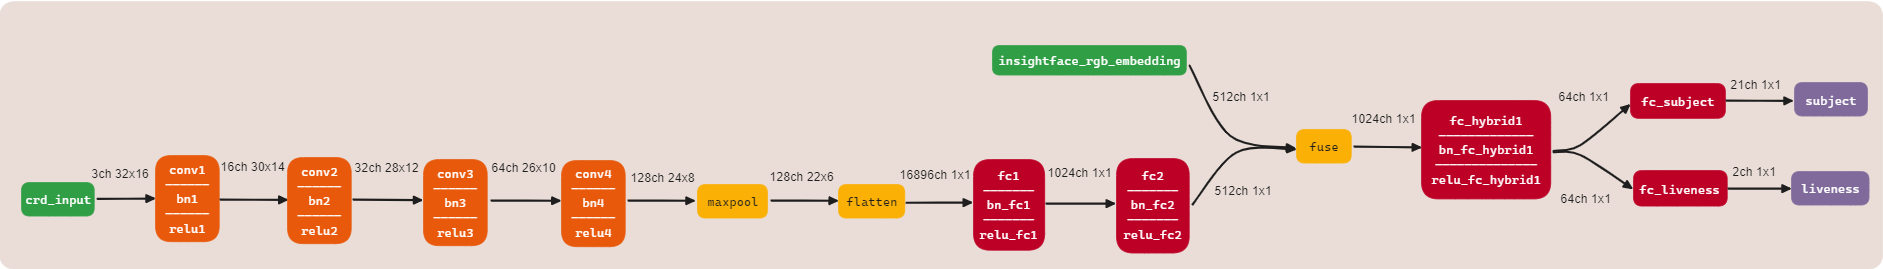
\includegraphics[width=1\textwidth]{diagrams/model_architecture.png}
    \caption{Architecture Diagram}
    \label{fig:model_architecture}
\end{figure*}


\section{Evaluation}

\subsection{Results}
% TODO: TABLE
% \begin{table}[htbp]
%     \centering
    
%     \begin{tabular}{lcccc}
%       \toprule
%       \multirow{2}{*}{\textbf{Feature Fusion}} & \multicolumn{2}{c}{\textbf{Subject}} & \multicolumn{2}{c}{\textbf{Liveness}} \\
%       \cmidrule(lr){2-3} \cmidrule(lr){4-5}
%        & \textbf{Accuracy} & \textbf{F1 Score} & \textbf{Accuracy} & \textbf{F1 Score} \\
%       \midrule
%       Concatenate & 83.70\% & 0.8347 & 99.60\% & 0.9932 \\
%       Add & 62.97\% & 0.6291 & 99.20\% & 0.9911 \\
%       Multiply & 87.10\% & 0.8543 & 96.66\% & 0.9481 \\
%       Pairwise Dot Average & 88.83\% & 0.8464 & 80.81\% & 0.7699 \\
%       Pairwise Dot Max & 82.70\% & 0.7905 & 72.84\% & 0.6962 \\
%       Pairwise Dot Flatten & 86.66\% & 0.8480 & 94.74\% & 0.9270 \\
%       Multi-Head Attention & 86.28\% & 0.7984 & 96.41\% & 0.8922 \\
%       \bottomrule
%     \end{tabular}
%     \caption{Results of Feature Fusion Techniques}
%     \label{tab:results}
%   \end{table}

%   \begin{table}[htbp]
%     \centering
%     \begin{tabular}{lcc}
%         \toprule
%         \textbf{Feature Fusion}   & \textbf{Macro-Averaged AUC} & \textbf{KL Divergence} \\
%         \midrule
%         Concatenate          & 0.7427                      & 0.9501                 \\
%         Add                  & 0.6672                      & 1.2934                 \\
%         Multiply             & 0.7282                      & 0.5468                 \\
%         Pairwise Dot Average & 0.9204                      & 0.2155                 \\
%         Pairwise Dot Max     & 0.8511                      & 0.2394                 \\
%         Pairwise Dot Flatten & 0.8562                      & 0.3653                 \\
%         Multi-Head Attention & 0.8229                      & 0.4775                 \\
%         \bottomrule
%     \end{tabular}
%     \caption{Performance Metrics for Feature Fusion Techniques}
%     \label{tab:metrics}
% \end{table}



\section{Conclusions}



\subsection{Future Work}


{\bf Acknowledgments.}
This is optional; it is a location for you to thank people, most probably your family and your supervisor.


\bibliographystyle{unsrt}
\bibliography{l5proj}

\end{document}
